\chapter{LHC Conditions, and Phenomenological Framework}

Since its formulation, the Standard Model (SM) has proven remarkably successful in describing the fundamental particles and interactions, and its parameters have been measured with increasing precision over several decades; however, as we have commented in the last chapter, various theoretical and experimental observations suggest that the SM is incomplete and certain details of the standard model seem to demand a better explanation, motivating the exploration of new physics (NP) beyond the standard model (BSM) and in turn methods in the search for this new physics. This pursuit requires both the development of theoretical models and the design of experimental strategies to test them. Particle physics phenomenology plays a crucial role in this endeavor by bridging theoretical predictions with experimental observations, feasibility and searches, particularly in high-energy experiments such as those conducted at the Large Hadron Collider (LHC), as well as in high-precision low-energy measurements.

The LHC is a proton-proton ($pp$) collider that has been operating since 2009, achieving center-of-mass collision energies ranging from $7~\mathrm{TeV}$ to $13.6~\mathrm{TeV}$. During its Run~I~(2010-2013), the LHC reached $7~\mathrm{TeV}$ in 2010-2011 and $8~\mathrm{TeV}$ in 2012, leading to landmark discoveries such as the Higgs boson in 2012. Run~II~(2015-2018) operated at $13~\mathrm{TeV}$ and achieved an instantaneous luminosity of $1.5 \times 10^{34}~\mathrm{cm}^{-2}~\mathrm{s}^{-1}$, yielding approximately 1000 top-quark pairs and 50 Higgs bosons per minute. Run~III~(2022-2025) is currently underway with collisions at a record energy of $13.6~\mathrm{TeV}$ and even higher luminosities. Following this, the High-Luminosity LHC (HL-LHC) is expected to begin operations around 2029. This major upgrade aims to increase the integrated luminosity by more than an order of magnitude, targeting up to $3\,\mathrm{ab}^{-1}$ of data per experiment. The HL-LHC will significantly enhance the sensitivity to rare processes, improve the precision of Standard Model measurements, and boost the discovery potential for BSM phenomena.

These collisions take place at four main interaction points, each equipped with a sophisticated particle detector designed to record and analyze the outcomes. Two of the largest and most comprehensive experiments at the LHC are the Compact Muon Solenoid (CMS) and ATLAS detectors. Both are multipurpose detectors with broad physics programs, designed to explore a wide range of phenomena. They perform precision measurements within the electroweak sector of the SM, investigate the dynamics of quarks and gluons (including through heavy-ion collisions), and carry out extensive searches for BSM signatures using $pp$ collision data. While CMS and ATLAS differ in their detector designs and reconstruction strategies, their physics goals are largely overlapping, and their results are complementary. Throughout this work, phenomenological studies and comparisons are primarily developed in the context of CMS, although several results from ATLAS are also referenced, given the close alignment in sensitivity and scope.

\section{Coordinate System and Collision Parameters}
To fully describe the CMS experiment, some of its parameters should be outlined. Measurements performed at CMS adopt the coordinate system whose origin lies at the collision point, with the $y$-axis pointing vertically upward, the $x$-axis pointing radially inward towards the centre of the LHC and the $z$-axis along the beam direction. The azimuthal angle $\phi$ is measured in the $x y$-plane from the $x$-axis and the polar angle, $\theta$, is measured from the $z$-axis, as shown in the Fig.~\ref{fig_coordinates}. 
\begin{center}
	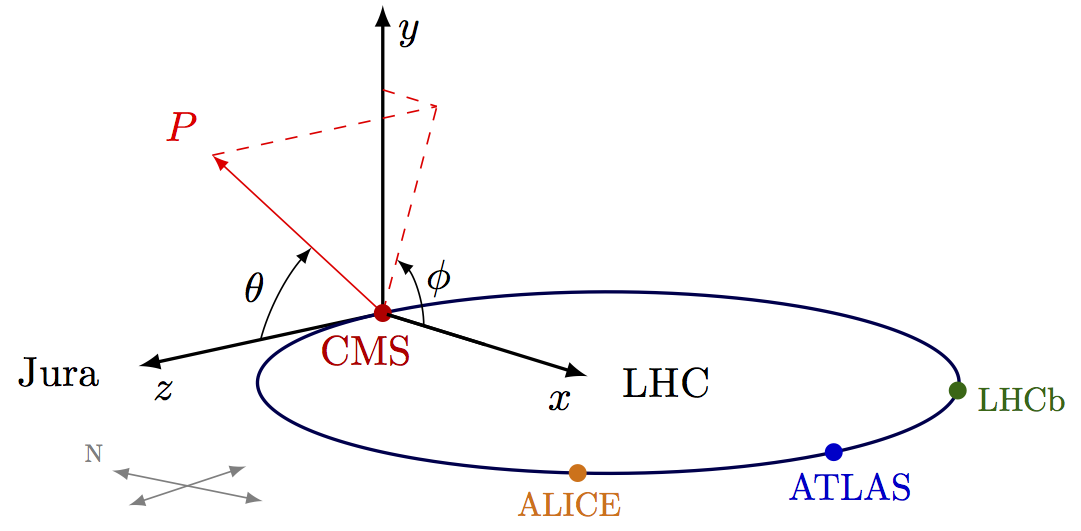
\includegraphics[width=0.80\textwidth]{Images/coordinatechart.png}
	\captionof{figure}{Coordinate system employed by the CMS experiment (retrieved from~\parencite{cmsplots}).}\label{fig_coordinates}
\end{center}
